\chapter{Results and Discussion}
\label{chap:evaluation}

A web application was developed which shows the results of the analysis applied on the data which got extracted and makes them accessible for everybody. Figure \ref{fig:start_page_prototype} shows the start page of this application.

\begin{figure}[h]
	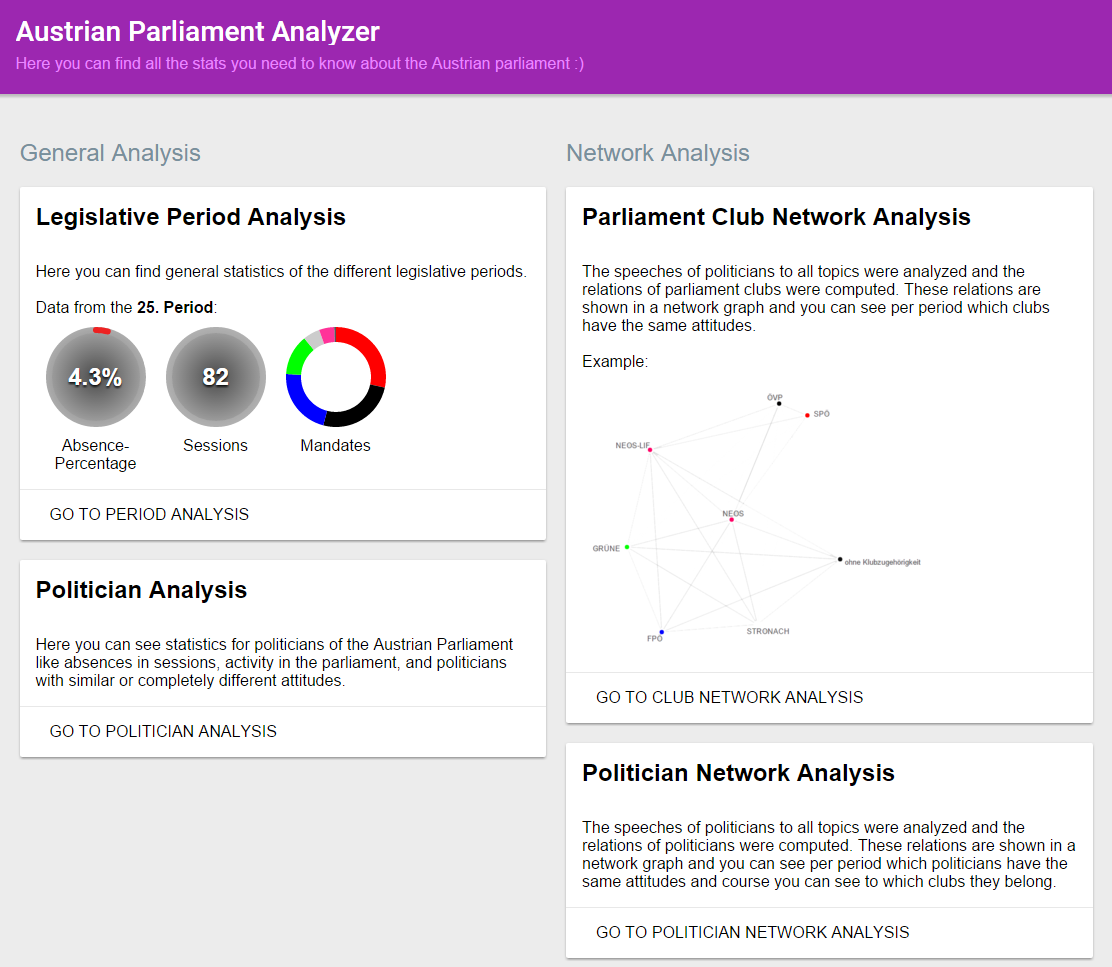
\includegraphics[width=\textwidth]{imgs/result_start_page}
	\caption{Start Page of the Prototype Web Application}
	\label{fig:start_page_prototype}
\end{figure}

\section{Relations of Parliament Clubs}
\label{sec:relations_clubs}
Figure \ref{fig:club_graphs1} shows the created relation graphs of the 25. and 22. legislative periods. The more positive the relation between two clubs is, the closer they appear together in the graph and the thicker is the edge between them. Only positive edges are shown in the graph, as the graph would be too confusing if the negative edges were also shown. In all graphs shown, one can easily see that there are two groups of parliamentary clubs in the parliament: Those which are in government and those which are in opposition. In table \ref{table:gov_opp_parties} the parties are listed per period weather they were in government or in opposition.

\begin{figure}
\begin{tabular}{ c  c }
	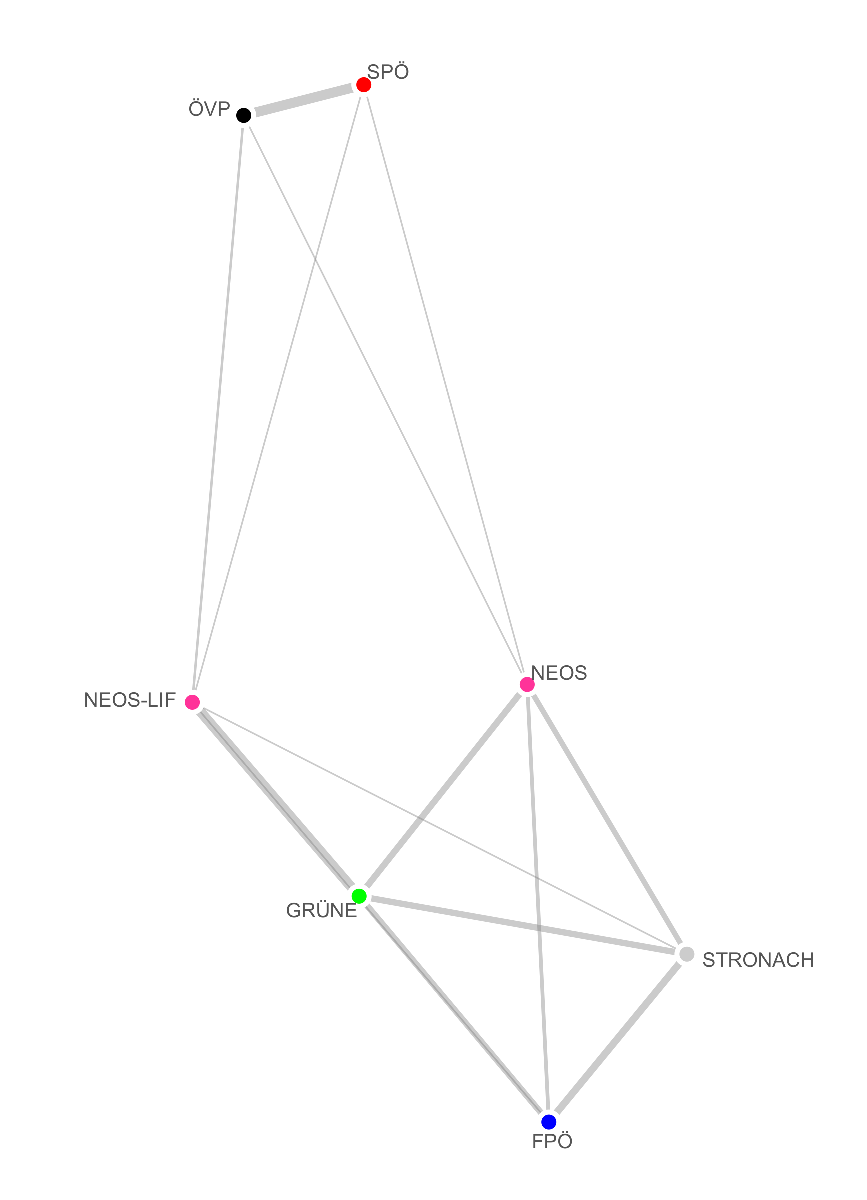
\includegraphics[width=0.47\textwidth]{imgs/graphs/club-graphs/graph_25.eps} 
	%& 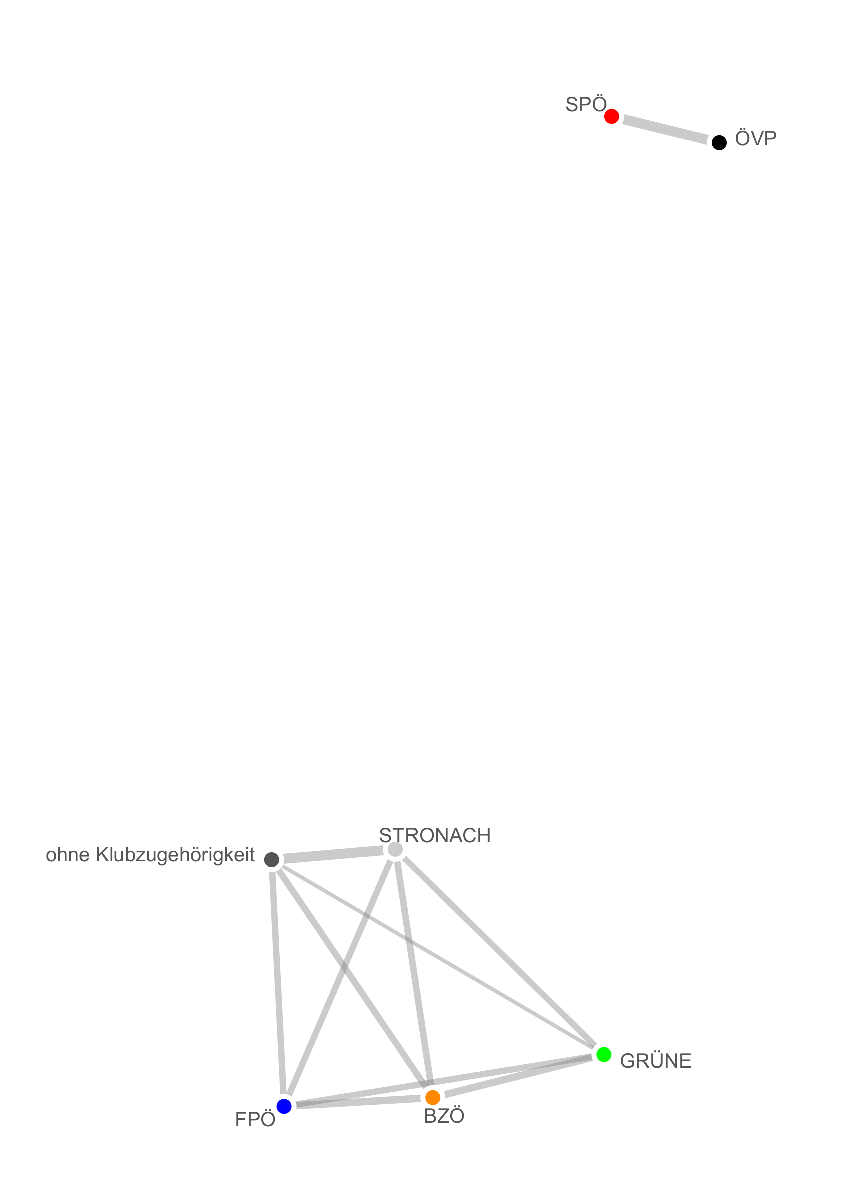
\includegraphics[width=0.3\textwidth]{imgs/graphs/club-graphs/graph_24.eps} 
	& 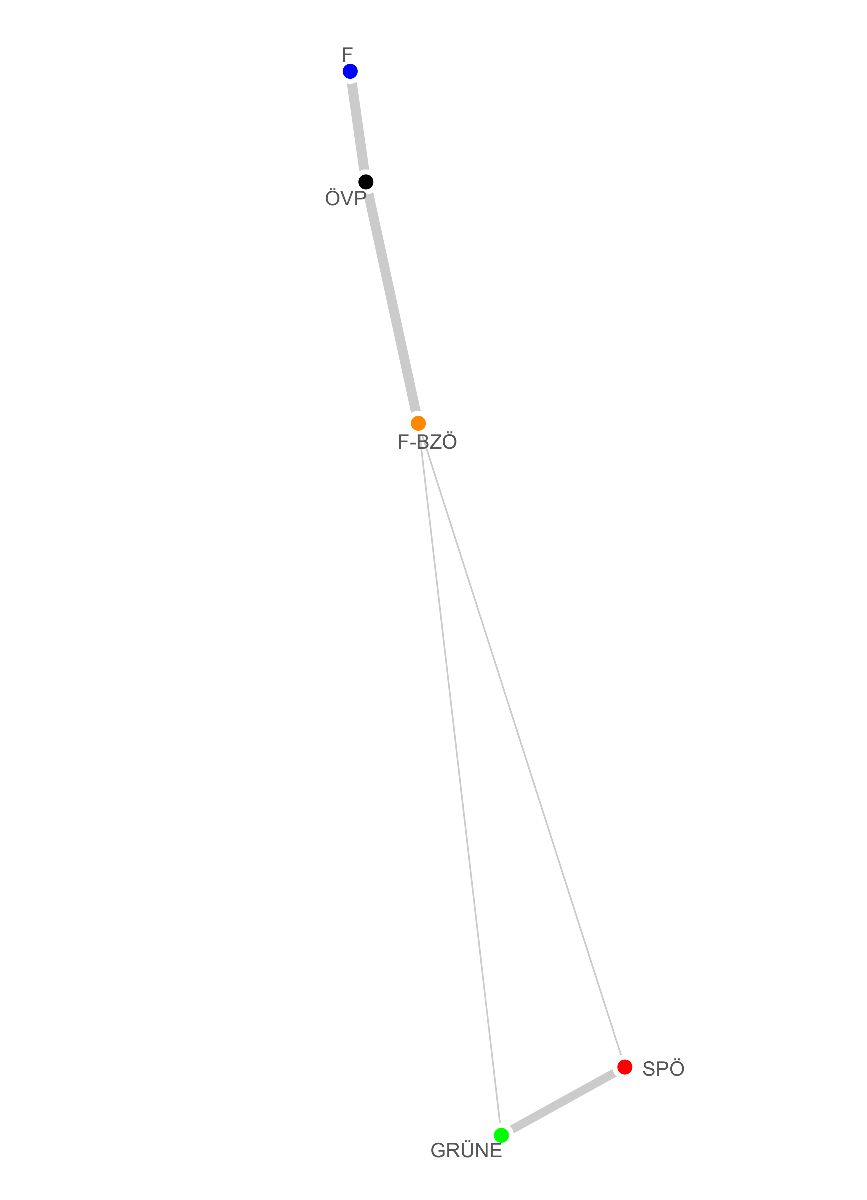
\includegraphics[width=0.47\textwidth]{imgs/graphs/club-graphs/graph_22.eps}
	\\
	(a) 25. Period 
	%& (b) 24. Period 
	& (c) 22.Period
\end{tabular}
	\caption{Club Relation Graph}
	\label{fig:club_graphs1}
\end{figure}

\begin{table}[h]

\centering
\bgroup
\def\arraystretch{1.2}
\begin{tabular}{| p{4cm} | p{3cm} | l |}
\hline
  Legislative Period & Governing Parties & Opposition  \\
\hline
\hline
  20. Period: 1995 - 1999 & SPÖ, ÖVP & FPÖ, Grüne, Liberale \\
\hline
  21. Period: 1999 - 2002 & ÖVP, FPÖ & SPÖ, Grüne \\
\hline
  22. Period: 2002 - 2006 & ÖVP, FPÖ, BZÖ\footnote{The BZÖ was in government from $17^{th}$ of April, 2005} & SPÖ, Grüne \\
\hline
  23. Period: 2006 - 2008 & SPÖ, ÖVP & FPÖ, Grüne, BZÖ \\
\hline
  24. Period: 2008 - 2013 & SPÖ, ÖVP & FPÖ, Grüne, Stronach, BZÖ \\
\hline
  25. Period: since 2013 & SPÖ, ÖVP & FPÖ, Grüne, NEOS, Stronach \\
\hline

\end{tabular}
\egroup
\caption{Government and Opposition in the Legislative Periods 20 to 25}
\label{table:gov_opp_parties}
\end{table}


\section{Relations of Politicians}
Graph + Explanations

\section{Government - Opposition Relation}
\label{sec:gov_opp_relation}


\begin{table}[h]

\centering
\bgroup
\def\arraystretch{1.2}
\begin{tabular}{| p{2cm} | p{3cm} | p{3cm} | p{3cm} |}
\hline
  Legislative Period & Government-Opposition Relation & Inner Government Relation & Inner Opposition Relation \\
\hline
\hline
  20. Period & -0.85 & +1.00 & +0.86 \\
\hline
  21. Period & -0.695 & +0.985 & +0.908 \\
\hline
  22. Period & -0.567 & +1.00 & +0.938 \\
\hline
  23. Period & -0.382 & +0.994 & +0.765\\
\hline
  24. Period & -0.52 & +1.00 & +0.768\\
\hline
  25. Period & -0.374 & +1.00 & +0.676\\
\hline

\end{tabular}
\egroup
\caption{Government-Opposition Relation, Inner Government- and Inner Opposition Relation for the Legislative Periods 20 to 25}
\label{table:gov_opp_relation}
\end{table}